\documentclass{mywork}
\addtolength{\headheight}{\baselineskip}
\lhead{Hauptseminar\\ \today}
\chead{Komplexe dynamische Systeme}
\rhead{\theauthor}
\renewcommand{\theta}{\vartheta}
\newcommand{\D}{\mathbb{D}}
\cfoot[LE,RO]{\bfseries\color{gray} -~\thepage~-}
\usepackage{pgfplots}
\usetikzlibrary{arrows,chains,matrix,positioning,scopes, shapes}
\begin{document}

\section{Motivation: das Newton-Verfahren}

Die Newtoniteration ist gegeben durch die Abbildung
\[
	\Phi(x)=z-\frac{f(z)}{f'(z)}.
\]
Dabei ist für einen Startwert $z_0$ folgendes Verhalten denkbar
\begin{itemize}
\item Die Newtoniteration konvergiert gegen eine Nullstelle von $f$,
\item Die Newtoniteration konvergiert nicht.
\end{itemize}

Das Newton-Verfahren konvergiert lokal. Wie ist das Konvergenzverhalten außerhalb dieser Konvergenzumgebung? In Abbildung 1 wurde das Konvergenzverhalten für gegebene Startwerte durch unterschiedliche Farben hervorgehebt. Vergleichen wir benachbarte Werte auf ihre Dynamik so stellen wir fest, dass es Punkte gibt in denen in keiner Umgebung alle Punkte diesselbe Dynamik besitzen.


\begin{figure}[H]
\centering
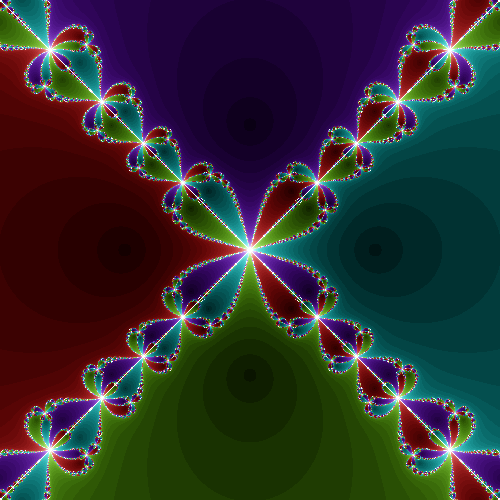
\includegraphics[scale=0.25]{fraktal.png}
\caption{Newton-Fraktal für $f(z)=z^4-1$}
\end{figure}


Dies motiviert das Konzept der \emph{Fatou-} bzw. \emph{Juliamenge}:
\begin{description}
\item[Fatou-Menge] Die Startwerte aus dieser Menge führen unter Iteration zu einer ,,stetigen`` Dynamik, das heißt, dass eine kleine Änderung des Startwert zu einer ähnlichen Dynamik führt.
\item[Julia-Menge] Beschreibt die Menge der Startpunkte, die zu den ,,instabilen`` Prozessen gehören. Jede noch so kleine Änderung des Startwerts führt zu einer komplett anderen Dynamik.
\end{description} 
Notation: $F(f)$ bezeichnet die Fatoumenge von $f$ und $J(f)$ analog die Juliamenge von $f$.


\section{Allgemeine Definitionen}

Sei im Folgenden $f: \overline{\C} \to \overline{\C}$ eine analytische Funktion auf $\C$ mit $f(\infty)=\infty$. Dabei setzen wir $f'(\infty)=\frac{d}{d z} \left [\frac{1}{f(1/z)} \right ](0)$. Weiterhin bezeichne $f^n$ die $n$-fache Verkettung von $f$.

\begin{df} \label{1}
Sei $z_0$ periodischer Punkt bzgl. $f$ mit Periode n, d.h. $f^n(z_0)=z_0$. Dann heißt er
\begin{itemize}
\item \emph{stark anziehend}, falls $|(f^n)'(z_0)|=0$,
\item \emph{anziehend}, falls $0<|(f^n)'(z_0)|<1$,
\item \emph{indifferent}, wenn $|(f^n)'(z_0)|=1$,
\item \emph{abstoßend}, wenn $|(f^n)'(z_0)|>1$.
\end{itemize} 
\end{df}


\begin{df}[Einzugsgebiet] \label{2}
Ist $z_0$ ein anziehender periodischer Punkt von $f$, dann ist die Menge
\[
	A_f(z_0)=\{z\in \overline{\mathbb{C}}: \exists_{L\subset \N} \, \lim\limits_{L\ni k\to \infty} f^{k}(z)=z_0\}
\]
das \emph{Einzugsgebiet} (engl. \emph{basin of attraction}) von $z_0$ bzgl. $f$.
\end{df}

\begin{df}[Julia-Menge] \label{3}
Wir definieren die Julia-Menge durch
\[
J(f):=\overline{\{z\in \overline{\mathbb{C}}: z \text{ abstossender periodischer Punkt von $f$} \}}
\]
Und die Fatou-Menge durch $F(f)=J(f)^c$
\end{df}


\section{Normale Familien und exzeptionelle Punkte}

\begin{df} \label{4}
Eine Familie $\{F_n\}$ analytischer Funktionen operiert \emph{normal} auf einer Umgebung $U$, falls jede Folge $(F_{n_i})_{i\in \mathbb{N}}$ eine Teilfolge $(F_{n_{i_j}})_{j\in \N}$ besitzt, sodass einer der beiden Eigenschaften erfüllt ist:
\begin{itemize}
\item $F_{n_{i_j}}$ konvergiert gleichmäßig auf kompakten Mengen $K\subset U$.
\item $F_{n_{i_j}}$ konvergiert gleichmäßig gegen $\infty$ auf $U$.
\end{itemize}
Eine Familie $\{F_n\}$ analytischer Funktionen operiert \emph{nicht normal} bei $z_0$, falls er in keiner Umgebung \emph{normal} operiert.
\end{df}



\begin{ex}\label{5}
Betrachte die Funktion $F$, gegeben durch $F(x)=ax$. Definiere die Familie $\{F^n\}$.

\textbf{Fall 1: $0<|a|<1$.} so konvergiert für jede kompakte Teilmenge die Funktionenfolge $F^n(z)=a^n\cdot z$ gleichmäßig gegen 0. Also operiert $\{F^n\}$ normal auf jeder Umgebung $U\subset \C$. 

$\longrightarrow J(f)=\{\infty\}, F(f)=\mathbb{C}$, $A_F(0)=\C$, $A_F(\infty)=\{\infty\}$.

\textbf{Fall 2: $|a|>1$.} Die Familie $\{F\}$ operiert nicht normal bei $0$, denn für $z\neq 0$ konvergiert jede beliebige Teilfolge gegen $\infty$. Nun konvergiert aber $F^{n_{i_j}}$ für beliebige Teilfolgen bei $z=0$ gleichmäßig gegen $0$.

$\longrightarrow J(F)=\{0\}$, $F(f)=\overline{\C}\setminus \{0\}$, $A(0)=\{0\}$, $A(\infty)=\bar{\C}\setminus \{0\}$. 
\end{ex}



\begin{prop}\label{6}
Sei $F$ analytisch, $z_0$ ein abstoßender periodischer Punkt bzgl. $F$. Dann operiert die Familie $\{F^n\}_{n\in \N}$ nicht normal bei $z_0$.
\end{prop}
\begin{proof}[Für Fixpunkte $z_0\in \C$]
 Angenommen $\{F^n\}$ operiert normal auf einer Umgebung $U$ von $z_0$. Für alle $n\in \N$ ist $F^n(z_0)=z_0$, also folgt insbesondere, dass $F^n$ nicht (gleichmäßig) gegen $\infty$ auf $U$ konvergiert. Also gibt es zu der Folge $(F^n)_{n\in \N}$ eine Teilfolge $(F^{n_i})_{i\in \N}$ die auf allen kompakten Teilmengen $K\subset U$ gleichmäßig konvergiert. Insbesondere ist die Grenzfunktion $G$ holomorph und es gilt $(F^{n_i})'(z_0) \to G'(z_0)$. Nun ist $z_0$ abstoßender Fixpunkt und damit folgt induktiv
 \[
 	|(F^{n_i})'(z_0)|=(F^{n_i-1} \circ F)'(z_0)|=|(F^{n_i-1})'(\underbrace{F(z_0)}_{=z_0})|\cdot |F'(z_0)| \stackrel{\text{ind.}}{=} \underbrace{|F'(z_0)|}_{>1} \stackrel{n\to \infty}\to \infty.
 \]
 Es ergibt sich der Widerspruch zur Beschränktheit von $\Big((F^{n_i})'(z_0)\Big)_{i\in \N}$.
\end{proof}



\begin{kor} \label{7}
Sei $F$ eine analytische Funktion. Die Familie $\{F^n\}_{n\in \N}$ operiert nicht normal für $z\in J(F)$.
\end{kor}

\begin{proof}
Die Menge der abstoßenden periodischen Punkte bzgl. $F$ liegt dicht in $J(F)$. Also finden wir in jeder Umgebung einen abstoßenden, periodischen Punkt bzgl. $F$. Nach Proposition~\ref{6} operiert $\{F^n\}$ nicht normal in sämtlichen Umgebungen von $z\in J(F)$. Insbesondere operiert $\{F^n\}$ nicht normal bei $z\in J(F)$.
\end{proof}

\begin{thm}[Montels Theorem] \label{8}
Sei $\{F_n\}$ eine Familie analytischer Funktionen auf einer Umgebung $U$. Angenommen es gibt $a,b \in \C, a\neq b$, sodass $F_n(z)\neq a \land F_n(z)\neq b$ für alle $n\in \N$ und $z\in U$. Dann operiert $\{F_n\}$ normal auf $U\subset \C$. (ohne Beweis) 
\end{thm}

\begin{kor} \label{9}
Sei $F$ eine analytische Funktion. Sei $z_0\in J(F)$ und sei $U$ eine beliebige Umgebung von $z_0$. Dann existiert höchstens ein $a\in \C$ mit
\[
	a\not\in \bigcup_{n=1}^\infty F^n(U).
\]
Wir nennen einen solchen Punkt \emph{exzeptionellen Punkt.}
\end{kor}

\begin{proof}
Angenommen es gibt $a\neq b, a,b \in \C$ mit $a,b \not\in \bigcup_{n=1}^\infty F^n(U)$. Also gilt für alle $n\in \N$ und für alle $z\in U$ $F^n(z)\neq a$ und $F^n(z)\neq b$. Aus Theorem \ref{8} (Montels Theorem) folgt, dass $\{F^n\}$ normal auf $U$ operiert. Nach Korollar \ref{7} operiert $\{F^n\}$ nicht normal bei $z_0$ und damit insbesondere auf $U$. Es ergibt sich der Widerspruch.
\end{proof}

\begin{thm}\label{10}
Sei $P$ ein Polynom mit Grad $\ge 2$. Angenommen es gibt einen Punkt $z_0\in J(P)$ samt einer Umgebung $U$ von $z_0$ und ein $a\in \C$, sodass 
\[
\bigcup_{n=0}^\infty P^{n}(U)=\C\setminus\{a\}
\]
so folgt $P(z)=a+\lambda(z-a)^k$ für $\lambda \in \C, k\in \N$ geeignet. 
Insbesondere ist $P$ mit Grad $n\ge 2$ topologisch konjugiert zu $Q: z \mapsto z^n$, d.h. 
das ein Homöomorphismus $H$ existiert mit $Q\circ H=H\circ P$.
\end{thm}

\begin{proof}
Wähle $b\in \C$, sodass $P(b)=a$. Es folgt, dass für beliebige $z\in U$ und $n\in \N$ folgt $P^n(z)\neq b$, denn sonst würde folgen $P^{n+1}(z)=P(b)=a$. Also ist $b$ ein exzeptioneller Punkt nach Korollar \ref{9} folgt $a=b$. Also ist $a\in \C$ Fixpunkt. Insbesondere ist $a$ das einzige Urbild von $a$, d.h. $P(b)\neq a$ für $b\neq a$, und es existiert ein $k\in \N$, sodass
\[
G(z)=\frac{P(z)-a}{(z-a)^k},
\] 
wobei $G$ ein Polynom mit $G(a)\neq 0$. Da $a$ einziger Fixpunkt von $P$ ist folgt $P(z)-a\neq 0$ für $z\neq a$ und insbesondere gilt
\[
G(z)=\frac{P(z)-a}{(z-a)^k}\neq 0, \text{ für } z \neq a.
\]
$G$ besitzt keine Nullstellen und ist nach dem Fundamentalsatz damit konstant $G\equiv \lambda\neq 0$. Also ist $P(z)=\lambda (z-a)^k+a$.

Definiere im Folgenden $H(z):=\sqrt[n]{\lambda}(z-a)$. Es ist leicht nachzurechnen, dass $Q\circ H=H\circ P$.
\end{proof}

\begin{ex} \label{11}
Für $Q(z)=z^n$, $n\ge 2$ folgt $J(Q)=S^1$. Sei $U$ eine Umgebung um $z_0\in S^1$ mit $0\not\in U$, dann folgt 
\[
0\not\in \bigcup_{k=0}^\infty Q^k(U).
\] 
Insbesondere ist $a=0$ exzeptioneller Punkt.
\end{ex}



\section{Periodische Punkte}

\begin{thm}[Koenigs Linearisationstheorem] \label{12}
Sei $f$ eine analytische Funktion mit $f(0)=0$ und $f'(0)=\lambda$ mit 
$|\lambda|\not\in\{0,1\}$, dann existiert ein Diffeomorphismus $\phi: U\to V$ mit 
$\phi(0)=0$, sodass 
\begin{align}
\phi \circ f(z)=\lambda\cdot \phi(z)  \label{*}\tag{$*$}
\end{align}
für $z\in U$, wobei $U$ und $V$ Umgebungen von $0$ sind. Dieses $\phi$ ist bis auf Multiplikation mit einer Konstanten eindeutig.
\end{thm}

\begin{proof}
\textbf{Eindeutigkeit:} Seien $\phi$ und $\psi$ analytische Funktionen die \eqref{*} erfüllen. Dann finden wir wegen Analyzität eine eindeutige Potenzreihendarstelung
\[
	\psi\circ \phi^{-1}(w)=\sum_{k=1}^\infty b_i w^i,\quad \psi\circ\phi^{-1}(0)=0.
\]
Es folgt
\[
\lambda \psi(\phi^{-1}(w))\stackrel{\lambda \psi = \psi \circ f} = \psi \circ f \circ \phi^{-1}(w)=\psi \circ \phi^{-1}\circ \phi \circ f \circ \phi^{-1}(w)\stackrel{\phi \circ f \circ \phi^{-1}=\lambda \cdot}= \psi \circ \phi^{-1}(\lambda w).
\]
Und damit
\[
	\sum_{k=1}^\infty \lambda b_i w^i=\lambda \psi \circ \phi^{-1}(w)=\psi \circ \phi^{-1}(\lambda w)= \sum_{k=1}^\infty b_i \lambda^i w^i.
\]
Mit Eindeutigkeit der Potenzreihendarstellung folgt $\lambda b_n=b_n \lambda^n$ für alle $n\in \N$ und wegen $|\lambda|\not\in \{0,1\}$ folgt $b_n=0$ für $n\ge 2$. Insbesondere ist
\[
\psi\circ\phi^{-1}(w)=b_1 w\text{, bzw. } \psi(z)=b_1 \phi(z).
\]
\textbf{Existenz: Fall $0<|\lambda|<1$.} Wähle $c<1$, sodass $c^2<|\lambda|<c$. Wähle $r>0$, sodass $|f(z)| \le c|z|$. Induktiv folgt $|f^n(z)|\le c^n r$. Mit Taylor folgt die Existenz einer Konstanten $k>0$, sodass $|f(z)-\lambda z|\le k |z|^2, |z|<r$. Es ist $|f(z)|\le c |z|\le c r< r$. So folgt
\[
|f^{n+1}(z)-\lambda f^n(z)|=|f(f^n(z))-\lambda f^n(z)|\le k |f^n(z)|^2\stackrel{\text{s.o.}}\le k c^{2n} r^2.
\]
Sei $\eps>0$ beliebig. Für hinreichend große $m,n$ ist
\[
	\Big|\frac{f^m(z)}{\lambda^m}-\frac{f^n(z)}{\lambda^n}\Big|=\Bigg|\sum_{i=n}^{m-1} \frac{f^{i+1}(z)}{\lambda^{i+1}}-\frac{f^i(z)}{\lambda^i}\Bigg|
	\le \sum_{i=n}^{m-1}\Big |\frac{f^{i+1}(z)}{\lambda^{i+1}}-\frac{f^i(z)}{\lambda^k}\Big | \stackrel{\text{s.o.}}\le \underbrace{\frac{k r^2}{|\lambda|}}_{:=k'} \sum_{i=n}^{m-1} \Bigg(\frac{c^2}{|\lambda|} \Bigg)^i< \eps.
\]
Und mit dem Cauchy-Kriterium für gleichmäßige Konvergenz, folgt dass $\Big(\frac{f^n}{\lambda^n}\Big)_{n\in \N}$ gleichmäßig konvergiert mit holomorpher Grenzfunktion $\phi$. Dabei gilt
\[
\phi(f(z))=\lim_{n\to \infty} \phi(f(z))=\lim_{n\to \infty} \frac{f^n(f(z))}{\lambda^n}= \lim_{n\to \infty} \lambda \underbrace{\frac{f^{n+1}(z)}{\lambda^{n+1}}}_{\to \phi(z)} = \lambda \phi(z).
\] 
Und es gilt
\[
\phi'(0)=\lim_{n\to \infty} \frac{(f^n)'(0)}{\lambda^n}\stackrel{\text{ind.}}= \lim_{n\to \infty} \frac{\prod_{i=0}^{n-1} f'(f^{i}(0))}{\lambda^n}\stackrel{f^{i}(0)=0}= \lim_{n\to \infty} \frac{f'(0)^n}{\lambda^n}=1.
\]
Also folgt aus dem Satz von der inversen Abbildung, dass die Abbildung $\phi$ eine Umgebung von $0$ diffeomorph abbildet und $\phi\circ f= \lambda\cdot \phi$.

\textbf{Fall $|\lambda|>1$.} Mit dem Satz von der Umkehrabbildung folgt, dass $f^{-1}$ lokal bei $z=0$ definiert ist, wobei
\[
|(f^{-1})'(0)|=\Bigg| \frac{1}{f'(f^{-1}(0))}\Bigg|\stackrel{f^{-1}(0)=0}= \frac{1}{|f'(0)|}=\lambda^{-1}<1.
\]
Mit obigem Argument folgt die Existenz von $\phi$ und einer Umgebung $U$ von 0 mit
\[
f^{-1}(z)=\phi^{-1}(\lambda^{-1}\phi(z)) \implies f(z)=\phi(\lambda \phi^{-1}(z)).
\]
für $z\in U$. Also gilt $\tilde \phi (f(z))=\lambda\cdot \tilde \phi(z)$, mit $\tilde \phi=\phi^{-1}$.
\end{proof}

\begin{prop} \label{13}
Sei $z_0$ ein anziehender periodischer Punkt bzgl. einer analytischen Funktion $f$, so existiert eine Umgebung $U$ um $z_0$, sodass $U\subset A_f(z_0)$. Wir nennen die Zusammenhangskomponente von $z_0\in A_f(z_0)$ auch das \emph{unmittelbare Einzugsgebiet} (engl. \emph{immediate basin of attraction}) von $z_0$ bzgl. $f$.
\end{prop}

\begin{proof} 
Sei $z_0$ anziehender periodischer Punkt mit Periode $m$. 
Setze $F(z):=f^m(z+z_0)-z_0$ für eine Umgebung von $0$. Offenbar gilt $F^n(z)=f^{nm}(z+z_0)-z_0$. Insbesondere ist $0$ anziehender Fixpunkt, denn 
\[
F^{n}(0)=\underbrace{f^{nm}(z_0)}_{=z_0}-z_0=0
\] 
mit $(F^{n})'(0)=(f^{mn})'(z_0)<1$. Nach Theorem~\ref{12} findet sich eine Umgebung $U'$ von $0$ und eine Abbildung $\phi$, so dass $F(z)=\phi^{-1}(\lambda\phi(z))$ und damit
\[
	f^{nm}(z+z_0)-z_0=F^n(z)=\phi^{-1}(\lambda^n \phi(z))
\]
Und es folgt
\[
\lim_{n\to \infty} f^{nm}(\underbrace{z+z_0}_{=:z'})\stackrel{\text{s.o.}}= \lim_{n\to \infty} \phi^{-1}(\lambda^n \phi(z))+z_0\stackrel{\text{Stet.}}= \phi^{-1}\Big(\lim_{n\to \infty} \lambda^n \phi(z)\Big)+z_0=\phi^{-1}(0)+z_0=z_0.
\]
für $z'\in z_0+U':=U$. Insbesondere gilt $U\subset A_f(z_0)$.
\end{proof}

%\begin{lem}
%Sei $|a|<1$. Definiere
%\[
%T_a(z):=\frac{z-a}{1-\bar a z}
%\]
%$T_a$ ist analytisch für $|z|<|a|^{-1}$. Desweiteren ist $T_a^{-1}=T_{-a}$, für $|z|<1$ und $T_a:\D\to \D$.
%\end{lem}

\begin{ex}
Sei $P$ ein Polynom vom Grad $n\ge 2$, dann ist $\infty$ ein stark anziehender Fixpunkt bzgl. $P$. Tatsächlich ist 
\[
|P'(\infty)|=\lim_{z\to 0}\Bigg|\frac{\mathrm{d}}{\mathrm{d}z}\Bigg[\frac{1}{P(1/z)}\Bigg]\Bigg|=\lim_{z\to 0}\Bigg|\frac{P'(1/z)}{z^2 P(1/z)^2}\Bigg|=\lim_{z\to 0} |z|^{n+1} \Bigg|\frac{z^{n-1} P'(1/z)}{z^{2n-2}z^2 P(1/z)^2}\Bigg|=0.
\]
\end{ex}

\begin{thm} \label{last}
Sei P ein Polynom vom Grad $n\ge 2$ und sei $z_0$ ein (stark) anziehender periodischer Punkt von $P$. Dann liegt im Einzugsgebiet von $z_0$ bzgl. $P$ ein kritischer Punkt.
\end{thm}

\begin{proof}
1) Setze $F(z)=P^m(z+z_0)-z_0$, wobei $m$ die Periode des anziehenden periodischen Punkts $z_0$ von $P$ ist. Im Beweis zu Proposition~\ref{13} wurde bereits gezeigt dass $0$ ein anziehender Fixpunkt ist.  Es genügt zu zeigen, dass $F$ im Einzugsgebiet von $0$ einen krtischen Punkt besitzt, denn sei $F'(z_{\mathrm{crit}})=0$, so folgt
\[
	\prod_{k=0}^{m-1} P'(P^{k-1}(z_{\mathrm{crit}}+z_0))=0.
\]
Also finden wir ein $k\in \{0,...,m-1\}$ mit $P'(P^k(z_{\mathrm{crit}}+z_0))=0$.

2) Angenommen $F'(0)=0$, dann sind wir fertig. Sei also $F'(0)\neq 0$. Wähle $r^*$, sodass $F(B_{r^*}(0))\subset B_{r^*}(0)$ injektiv und $B_{r*}(0)$ im Einzugsgebiet von $0$ bzgl. $F$ liegt. Dies lässt sich so realisieren wegen dem Satz von der lokalen Umkehrabbildung und Proposition~\ref{13}. Setze nun $V:=F^{-1}(B_{r^*}(0))$. Dann wird $F$ als Abbildung von $V$ nach $U$ surjektiv.

\textbf{Behauptung:} Falls $F$ keine kritischen Punkte in $B_{r^*}(0)$ besitzt, so besitzt $F$ eine analytische Umkehrabbildung $F^{-1}: B_{r^*}(0) \to U$, sodass $U\subset V$ ein Gebiet und $F^{-1}(0)=0$.

\textbf{Beweis.} Nach Konstruktion existiert ein analytisches Inverse $F^{-1}: F(B_{r^*}(0)) \to B_{r^*}(0)$. Also können wir $F^{-1}$ über Wege von $0$ durch lokale Umkehrfunktionen analytisch fortsetzen.

\begin{figure}[H]
\centering
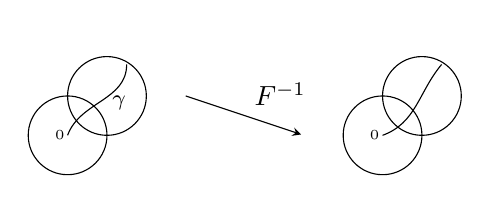
\begin{tikzpicture}
\draw (-.1,0) node{\tiny{$0$}} (0,0)  circle (.5) (.5,.5) circle (.5) (1, 1.25) node {$\iddots$}; 
\draw[->,>=stealth,shorten >=1pt,auto,node distance=3cm] (1.5,.5) -- node{$F^{-1}$} (3,0);
\draw (3.9,0) node{\tiny{$0$}} (4,0) circle (.5) (4.5,.5) circle(.5) (5, 1.25) node {$\iddots$};
\path[auto, node distance=3cm] (0,0) edge [out=70, in=-90] node[near end, below]{\footnotesize{$\gamma$}} (.75,.9);
\path (4,0) edge [out=20, in=-130] (4.75,.9);
\end{tikzpicture}
\end{figure}

Dadurch erhalten wir eine analytische Abbildung $F^{-1}: B_{r^*}(0) \to U$, die surjektiv ist. Diese ist mit dem Monodromiesatz wohldefiniert. Es bleibt zu zeigen, dass $F^{-1}$ injektiv ist. Angenommen $F^{-1}(z_1)=F^{-1}(z_2)$. Dann ist $F(F^{-1}(z_1))=F(F^{-1}(z_2))$ und da $F^{-1}$ gerade lokal die Umkehrabbildung beschreibt auch $z_1=z_2$.

3) Angenommen im Einzugsgebiet von $0$ bzgl. $F$ gibt es keine kritischen Punkte, so können wir $F^{-1}$ auf sukzessiv größer werdenden Gebieten definieren, die selbst wieder im Einzugsgebiet sind. Dabei gilt
\[
\bigcup_{k\in \N_0} F^{-k}(B_{r^*}(0))\subset \C\setminus \{z| |z|>R\}
\] 
für hinreichend großes $R>r^*$. Tatsächlich gilt für $R$  hinreichend groß $|F(z)| \ge |z|$ und insbesondere folgt damit auch $|F^n(z)|>R>r^*$ für alle $n\in \N$. 

Nach Konstruktion gilt dabei 
\[
|(F^{-k})'(0)|=\Bigg|\frac{1}{(F^k)'(F^{-k}(0))} \Bigg|\stackrel{F^{-k}(0)=0}= \frac{1}{|(F^k)'(0)|}>1.
\]
Also ist $0$ ein abstoßender Fixpunkt bzgl. $F^{-1}$. Nach Korollar~\ref{9} gibt es aber höchstens einen exzeptionellen Punkt. Es ergibt sich der Widerspruch. Also finden wir im Einzugsgebiet von $0$ bzgl. $F$ einen kritischen Punkt. Mit dem vorigen Resultat folgt, dass im Einzugsgebiet von $z_0$ bzgl. $P$ ein kritischer Punkt zu finden ist.
\end{proof}

\end{document}
